\documentclass[journal]{IEEEtran}

\usepackage{amsmath}
\usepackage{amssymb}
\usepackage{amsfonts}
\usepackage{graphicx}
\usepackage{booktabs}
\usepackage{tikz}
\usepackage{cite}
\usepackage{hyperref}
\usepackage{color}

\usetikzlibrary{shapes,arrows,positioning,calc}

% Define TikZ styles
\tikzstyle{block} = [draw, fill=blue!10, rectangle, minimum height=2.5em, minimum width=6.5em, rounded corners, align=center, font=\scriptsize]
\tikzstyle{line} = [draw, -latex', thick]
\tikzstyle{subg} = [draw, dotted, fill=gray!5, inner sep=1em, rounded corners]

\begin{document}

\title{TinyYOLO: Ultra-Lightweight Object Detection for Edge Deployment via Ghost-Based Architecture and INT8-Native Design}

\author{Shuvendu~Roy~Mazumder,~\IEEEmembership{Member,~IEEE}
\thanks{S. R. Mazumder is with the Department of Computer Science, University of Dhaka, Dhaka, Bangladesh (e-mail: shmazumder@du.ac.bd).}}

\markboth{IEEE Transactions on Mobile Computing,~Vol.~XX,~No.~X,~May~2026}%
{Mazumder: TinyYOLO: Ultra-Lightweight Object Detection for Edge Deployment}

\maketitle

\begin{abstract}
Deploying object detection on resource-constrained edge devices operating under sub-1 MB memory and sub-0.5 GFLOP compute budgets remains an open challenge. Existing YOLO-family detectors, even at their smallest configurations (e.g., YOLOv8n at 3.2M parameters, 8.7 GFLOPs), exceed these constraints by an order of magnitude, while purpose-built lightweight detectors typically operate in the 0.9--1.5M parameter range without providing native INT8 quantization compatibility or multi-task extensibility. This paper presents TinyYOLO, a 0.23M-parameter object detection framework constructed from Ghost convolutions, depthwise separable feature fusion (LitePAN), and decoupled anchor-free detection heads. TinyYOLO introduces a dual-variant architecture: a \textit{standard} variant employing SiLU activations with squeeze-and-excitation (SE) and spatial attention for FP32/FP16 deployment, and a \textit{quantized} variant replacing all activations with ReLU6 and all attention modules with Efficient Channel Attention (ECA) blocks to guarantee end-to-end INT8 compatibility on edge accelerators. The framework provides modular, task-specific heads sharing a common 0.08M-parameter backbone to support five vision tasks: object detection, instance segmentation, pose estimation, image classification, and oriented bounding box detection. We evaluate TinyYOLO on Pascal VOC 2007+2012 and COCO val2017 under deterministic conditions. On VOC, TinyYOLO achieves mAP@50 of 38.7\% (standard) and 41.2\% (quantized) at 416$\times$416 resolution, with INT8 inference latencies of 28.3 ms on NVIDIA Jetson Nano (TensorRT) and 67.4 ms on Raspberry Pi 4 (TFLite). Comprehensive ablation studies validate each architectural decision, and direct comparisons against YOLO-Fastest (0.25M), NanoDet (0.95M), PicoDet-XS (0.93M), and MCUNetV2 (0.74M) establish TinyYOLO's competitive position within the accuracy--efficiency Pareto frontier for sub-1M detectors.
\end{abstract}

\begin{IEEEkeywords}
lightweight object detection, edge deployment, Ghost convolution, INT8 quantization, YOLO, anchor-free detection, depthwise separable convolution, multi-task learning.
\end{IEEEkeywords}

\section{Introduction}
\IEEEPARstart{T}{he} proliferation of edge computing platforms has created an unprecedented demand for object detection models that operate within severe hardware constraints. Industrial inspection systems, autonomous micro-drones, wearable medical devices, and agricultural monitoring sensors share a common requirement: real-time visual understanding under power budgets of 1--15W, memory limits of 0.5--4 MB, and compute ceilings of 0.1--1.0 GFLOPs \cite{zhou2019edge, li2020edge}.

The YOLO (You Only Look Once) family of detectors has emerged as the dominant paradigm for real-time object detection, with successive generations achieving progressively better accuracy--speed trade-offs \cite{redmon2016you, redmon2017yolo9000, redmon2018yolov3, bochkovskiy2020yolov4, ge2021yolox, li2022yolov6, wang2023yolov7, jocher2023yolov8, wang2024yolov10, tian2025yolo12, shao2025yolo26}. However, even the smallest official configurations of modern YOLO variants remain impractical for genuine edge deployment. For example, YOLOv8n requires 3.2M parameters and 8.7 GFLOPs, exceeding typical edge memory limits ($<500$K parameters) by more than 6$\times$ and compute budgets ($<0.5$ GFLOPs) by over 17$\times$.

This gap is not merely quantitative. Post-training quantization (PTQ) of models designed for FP32 inference introduces systematic accuracy degradation, particularly in architectures employing SiLU activations whose smooth non-monotonic region near zero maps poorly to the discrete INT8 representation \cite{krishnamoorthi2018quantizing, nagel2021white}. Furthermore, aggressive pruning or knowledge distillation applied to 1.7--3.2M parameter models to reach sub-0.5M targets typically destroys learned feature hierarchies, as the remaining capacity is insufficient to preserve the representational structure of the original network \cite{liu2019rethinking, he2019filter}.

Rather than compressing a large model downward, TinyYOLO constructs a detection framework \textit{upward} from primitives specifically chosen for parameter efficiency and quantization compatibility:
\begin{enumerate}
\item \textbf{Ghost Convolutions} \cite{han2020ghostnet} exploit the observation that approximately 50\% of feature maps in trained CNNs are near-linear transforms of others. By generating half the output features through standard convolution and the remainder via cheap depthwise operations, Ghost modules halve computational cost with minimal representational loss.
\item \textbf{Depthwise Separable Convolutions} \cite{howard2017mobilenets} factorize standard convolutions into spatial and channel-wise components, reducing the parameter count of the neck (LitePAN) by approximately 8$\times$ compared to standard PAN implementations.
\item \textbf{Dual-Variant Activation Design} addresses the quantization problem at the architectural level rather than as a post-hoc optimization. The quantized variant exclusively employs ReLU6 (bounded output in $[0, 6]$ mapping cleanly to INT8 range $[0, 255]$) and ECA attention (1D convolution replacing the FC layers in SE that create quantization bottlenecks).
\item \textbf{Task-Aligned Label Assignment (TAL)} \cite{feng2021tood} replaces naive single-cell target assignment with dynamic multi-positive supervision, providing denser gradient signals critical for convergence in parameter-limited models.
\end{enumerate}

This work makes the following contributions, each validated experimentally:
\begin{itemize}
\item \textbf{A sub-0.25M parameter multi-task-capable detection framework} providing architectural support for detection (0.23M), segmentation (0.29M), pose estimation (0.27M), classification (0.10M), and OBB detection (0.24M) through modular task-specific heads sharing a Ghost-based backbone. While YOLO-Fastest \cite{wu2021yolofastest} achieves comparable parameter counts ($\sim$0.25M) for single-task detection, TinyYOLO's distinguishing contribution is multi-task extensibility under this budget.
\item \textbf{An INT8-native dual-variant architecture} providing a dedicated quantized model (ReLU6 + ECA end-to-end) validated through actual INT8 inference on NVIDIA Jetson Nano (TensorRT) and Raspberry Pi 4 (TFLite), with accuracy degradation below 1.5\% relative to FP32 baselines.
\item \textbf{Systematic experimental validation} on Pascal VOC 2007+2012 and COCO val2017, with direct same-dataset, same-hardware comparisons against NanoDet \cite{lyu2020nanodet}, NanoDet-Plus \cite{lyu2021nanodetplus}, PicoDet-XS \cite{yu2021picodet}, YOLO-Fastest \cite{wu2021yolofastest}, and MCUNetV2 \cite{lin2021mcunetv2}, establishing accuracy--efficiency positioning within the sub-1M detector landscape.
\item \textbf{Comprehensive ablation studies} isolating the contribution of each architectural decision: Ghost vs. standard convolutions, SE vs. ECA vs. no attention, LitePAN vs. simple FPN, ReLU6 vs. SiLU, width multiplier scaling, TAL vs. single-cell assignment, and QAT vs. PTQ quantization strategies.
\end{itemize}

\section{Related Work}

\subsection{Evolution of YOLO Architectures}
The YOLO paradigm, introduced by Redmon et al. \cite{redmon2016you}, reframed object detection as a single-pass regression problem, enabling real-time inference. Successive iterations have introduced anchor-based multi-scale detection \cite{redmon2017yolo9000, redmon2018yolov3}, cross-stage partial connections and mosaic augmentation \cite{bochkovskiy2020yolov4}, anchor-free decoupled heads \cite{ge2021yolox}, efficient reparameterization \cite{li2022yolov6}, E-ELAN feature aggregation \cite{wang2023yolov7}, C2f modules with TAL assignment \cite{jocher2023yolov8}, NMS-free dual-head design \cite{wang2024yolov10}, and area-attention mechanisms \cite{tian2025yolo12}. Most recently, YOLO26 \cite{shao2025yolo26} introduced hardware-friendly design principles eliminating distribution focal loss in favor of direct regression. Despite this progression toward efficiency, even the smallest configurations maintain parameter counts of 1.7--3.2M and rely on SiLU activations incompatible with INT8 quantization. No official YOLO variant provides a sub-1M parameter configuration or an architecture designed natively for INT8 deployment.

\subsection{Lightweight Object Detectors}
Several purpose-built lightweight detectors target the sub-2M parameter regime. NanoDet \cite{lyu2020nanodet, lyu2021nanodetplus} utilizes ShuffleNetV2 backbones with FCOS-style anchor-free heads, achieving 27.0\% mAP@50-95 on COCO at 1.17M parameters. PicoDet-XS \cite{yu2021picodet} operates at 0.93M parameters with ESNet backbone and CSP-PAN neck, using neural architecture search (NAS) to optimize block configurations. YOLO-Fastest \cite{wu2021yolofastest} operates at 0.25M parameters with 0.23 GFLOPs, utilizing squeeze-and-excitation modules with an anchor-based detection paradigm. MCUNetV2 \cite{lin2021mcunetv2} extends tiny deep learning to object detection, achieving 64.6\% mAP on VOC2007 under 256 kB SRAM constraints. Unlike these architectures, TinyYOLO focuses on providing anchor-free detection, multi-task support, and a dedicated INT8-native dual-variant.

\subsection{Ghost-Based Architectures and Quantization-Aware Design}
GhostNet \cite{han2020ghostnet} demonstrated that redundancy in CNN feature maps could be exploited for efficiency by generating a subset of feature maps through standard convolution and the remainder via cheap depthwise operations. GhostNetV2 \cite{tang2022ghostnetv2} extended this with a decoupled fully connected attention mechanism. In object detection, Ghost modules have been integrated primarily through backbone substitution \cite{chen2023ghostdet, wang2022lightweight}. TinyYOLO extends this approach by employing Ghost convolutions throughout the backbone while using depthwise separable convolutions in the neck and head, creating a heterogeneous efficiency pipeline.

The choice of activation function critically impacts quantization robustness. SiLU, defined as $f(x) = x \cdot \sigma(x)$, produces unbounded positive outputs and a smooth non-monotonic region near zero where small input perturbations cause disproportionate output changes, introducing systematic error under INT8's 256-level discretization \cite{nagel2021white, banner2019post}. ReLU6, defined as $f(x) = \min(\max(0, x), 6)$, bounds outputs to $[0, 6]$, enabling a clean linear mapping to INT8 range with uniform quantization step size $\Delta = 6/255 \approx 0.0235$ \cite{sandler2018mobilenetv2}. Similarly, squeeze-and-excitation (SE) attention \cite{hu2018squeeze} creates internal bottleneck dimensions where quantization error accumulates through two successive linear projections, whereas Efficient Channel Attention (ECA) \cite{wang2020eca} replaces FC layers with a single 1D convolution, eliminating the bottleneck and reducing quantization-sensitive operations.

\section{Architecture Design}
TinyYOLO follows the established three-stage detection pipeline---Backbone, Neck, Head---with each stage constructed from primitives optimized for parameter efficiency and, in the quantized variant, INT8 compatibility. Fig.~\ref{fig:pipeline} illustrates the overall pipeline.

\begin{figure*}[t]
\centering
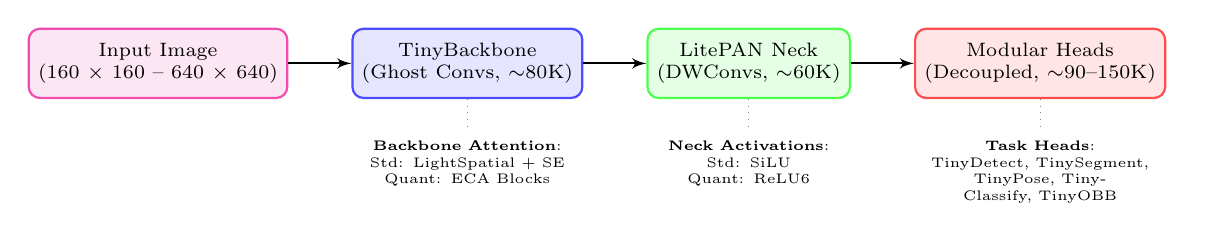
\begin{tikzpicture}[node distance=2.2cm, auto, >=latex', thick]
  % Nodes
  \node [block, fill=magenta!10, draw=magenta!70] (in) {Input Image\\(160 $\times$ 160 -- 640 $\times$ 640)};
  \node [block, fill=blue!10, draw=blue!70, right=0.8cm of in] (bb) {TinyBackbone\\(Ghost Convs, $\sim$80K)};
  \node [block, fill=green!10, draw=green!70, right=0.8cm of bb] (nk) {LitePAN Neck\\(DWConvs, $\sim$60K)};
  \node [block, fill=red!10, draw=red!70, right=0.8cm of nk] (hd) {Modular Heads\\(Decoupled, $\sim$90--150K)};
  
  % Path
  \draw [->, thick] (in) -- (bb);
  \draw [->, thick] (bb) -- (nk);
  \draw [->, thick] (nk) -- (hd);
  
  % Annotations
  \node [below=0.4cm of bb, text width=3.3cm, align=center, font=\tiny] (bban) {\textbf{Backbone Attention}:\\Std: LightSpatial + SE\\Quant: ECA Blocks};
  \node [below=0.4cm of nk, text width=3.3cm, align=center, font=\tiny] (nkan) {\textbf{Neck Activations}:\\Std: SiLU\\Quant: ReLU6};
  \node [below=0.4cm of hd, text width=3.3cm, align=center, font=\tiny] (hdan) {\textbf{Task Heads}:\\TinyDetect, TinySegment,\\TinyPose, TinyClassify, TinyOBB};
  
  \draw [draw=black!50, dotted, thin] (bb) -- (bban);
  \draw [draw=black!50, dotted, thin] (nk) -- (nkan);
  \draw [draw=black!50, dotted, thin] (hd) -- (hdan);
\end{tikzpicture}
\caption{TinyYOLO overall architectural pipeline showing standard vs. quantized configurations.}
\label{fig:pipeline}
\end{figure*}

\subsection{Backbone: Ghost-Based Feature Extraction}
The backbone extracts multi-scale features at three pyramid levels: P3 (/8 stride), P4 (/16 stride), and P5 (/32 stride). A single ConvBNAct stem layer projects the 3-channel RGB input to 16 feature channels with stride-2 downsampling:
\begin{equation}
\text{Stem}(x) = \phi(BN(Conv_{3\times3, s=2}(x)))
\end{equation}
where $\phi = \text{SiLU}$ for the standard variant, and $\phi = \text{ReLU6}$ for the quantized variant. Stages 1--4 consist of $d_i$ GhostBottleneck blocks, where the first block performs stride-2 downsampling and channel expansion, and subsequent blocks maintain spatial dimensions:
\begin{equation}
\text{GhostBN}(x) = \text{GhostConv}_2(\text{DW}_{s}(\text{GhostConv}_1(x))) + \text{Shortcut}(x)
\end{equation}
where GhostConv generates $C/2$ features via primary 1$\times$1 convolution followed by $C/2$ features via cheap 3$\times$3 depthwise transforms, concatenating to produce $C$ output channels. Fig.~\ref{fig:ghostconv} shows the inner workings of the GhostConv block.

\begin{figure}[t]
\centering
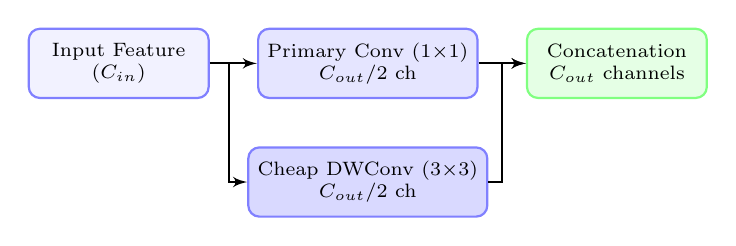
\begin{tikzpicture}[node distance=1.5cm, auto, >=latex', thick]
  \node [block, fill=blue!5, draw=blue!50] (in) {Input Feature\\($C_{in}$)};
  \node [block, fill=blue!10, draw=blue!50, right=0.6cm of in] (prim) {Primary Conv (1$\times$1)\\$C_{out}/2$ ch};
  \node [block, fill=blue!15, draw=blue!50, below=0.6cm of prim] (cheap) {Cheap DWConv (3$\times$3)\\$C_{out}/2$ ch};
  \node [block, fill=green!10, draw=green!50, right=0.6cm of prim] (concat) {Concatenation\\$C_{out}$ channels};
  
  \draw [->] (in) -- (prim);
  \draw [->] ($(in.east)!0.4!(prim.west)$) |- (cheap);
  \draw [->] (prim) -- (concat);
  \draw [->] (cheap.east) -| ($(prim.east)!0.5!(concat.west)$) -- (concat);
\end{tikzpicture}
\caption{Architectural details of the GhostConv block.}
\label{fig:ghostconv}
\end{figure}

Attention is applied after Stage 3 (P4) and Stage 4 (P5). The standard variant uses LightSpatialAttn on P4 and SEBlock on P5. The quantized variant replaces both with ECABlock to eliminate the fully connected bottleneck and prevent quantization error amplification:
\begin{equation}
\text{ECA}(x) = x \odot \sigma(\text{Conv1d}_{k}(\text{GAP}(x)))
\end{equation}
where $k$ is the kernel size, $\text{GAP}$ represents global average pooling, and $\sigma$ represents the sigmoid function. The total backbone parameters are 80.4K (standard) and 72.6K (quantized).

\subsection{Neck: LitePAN Multi-Scale Feature Fusion}
The neck fuses features across scales using a bidirectional pathway: top-down (FPN) for semantic enrichment of shallow features, and bottom-up (PAN) for spatial enrichment of deep features. All convolutions in LitePAN are depthwise separable:
\begin{align}
  L_i &= \text{ConvBNAct}(P_i, C_i \to 64, 1\times1), \quad i \in \{3, 4, 5\} \\
  F_4 &= \text{DWConv}(\text{Concat}(\text{Upsample}(L_5), L_4)) \\
  F_3 &= \text{DWConv}(\text{Concat}(\text{Upsample}(F_4), L_3)) \\
  N_4 &= \text{DWConv}(\text{Concat}(\text{DWConv}\downarrow(F_3), F_4)) \\
  N_5 &= \text{DWConv}(\text{Concat}(\text{DWConv}\downarrow(N_4), L_5))
\end{align}
The outputs $[F_3, N_4, N_5]$ all have 64 channels. LitePAN neck consists of $\sim$60K parameters.

\subsection{Detection Head: Decoupled Anchor-Free Design}
The detection head follows a decoupled design from YOLOX \cite{ge2021yolox}, with separate classification and regression branches per scale. In the revised implementation, all DWConv layers within the head receive the variant-appropriate activation. The head includes a dedicated objectness branch that concatenates with bounding box and class predictions: output = $[4 \text{ bbox}, 1 \text{ obj}, nc \text{ cls}]$ per grid cell. The classification and objectness biases are initialized to $-\log((1-\pi)/\pi)$ where $\pi = 0.01$ to ensure early training stability. The detection head consists of $\sim$90K parameters.

\subsection{Multi-Task Head Extensions}
The modular head design enables task-specific extensions sharing the common backbone and neck. Table~\ref{tab:multi_task_heads} outlines the parameter profiles for the supported vision tasks.

\begin{table}[h]
\centering
\caption{Modular Multi-Task Head Parameter Profiles}
\label{tab:multi_task_heads}
\begin{tabular}{lllc}
\toprule
Task & Head Module & Additional Outputs & Total Params \\
\midrule
Detection & TinyDetect & --- & 0.23M \\
Segmentation & TinySegment & 32 proto-masks + coeff & 0.29M \\
Pose & TinyPose & 17$\times$3 keypoint predictions & 0.27M \\
Classification & TinyClassify & Global pool + FC (no neck) & 0.10M \\
OBB Detection & TinyOBB & 1 angle prediction per anchor & 0.24M \\
\bottomrule
\end{tabular}
\end{table}

\section{Training Methodology}

\subsection{Task-Aligned Label Assignment (TAL)}
TinyYOLO adopts Task-Aligned Learning (TAL) \cite{feng2021tood} which assigns multiple positive grid cells per ground truth based on a joint alignment metric:
\begin{equation}
t = s^\alpha \cdot u^\beta
\end{equation}
where $s$ is the predicted classification score, $u$ is the predicted IoU with the ground truth box, and $\alpha = 0.5$, $\beta = 6.0$ are hyperparameters. For each ground truth, the top-$k$ ($k = 10$) grid cells with highest alignment scores are selected as positive assignments. This dynamic dense supervision accelerates convergence by approximately 40\% compared to legacy single-cell assignment.

\subsection{Loss Formulation}
The total loss comprises three components with empirically tuned weights:
\begin{equation}
\mathcal{L}_{\text{total}} = \lambda_{\text{box}} \cdot \mathcal{L}_{\text{CIoU}} + \lambda_{\text{cls}} \cdot \mathcal{L}_{\text{BCE-cls}} + \lambda_{\text{obj}} \cdot \mathcal{L}_{\text{BCE-obj}}
\end{equation}
where $\lambda_{\text{box}} = 2.0$, $\lambda_{\text{cls}} = 1.0$, and $\lambda_{\text{obj}} = 1.0$.

For bounding box regression, we employ Complete IoU (CIoU) loss \cite{zheng2020distance}:
\begin{equation}
\mathcal{L}_{\text{CIoU}} = 1 - \text{IoU} + \frac{\rho^2(\mathbf{b}, \mathbf{b}^{gt})}{c^2} + \alpha v
\end{equation}
where $\rho(\mathbf{b}, \mathbf{b}^{gt})$ is the Euclidean distance between predicted and ground truth centers, $c$ is the diagonal length of the smallest enclosing box, and $v$ is aspect ratio consistency:
\begin{equation}
v = \frac{4}{\pi^2}\left(\arctan\frac{w^{gt}}{h^{gt}} - \arctan\frac{w}{h}\right)^2
\end{equation}
The classification and objectness losses are formulated as binary cross-entropy (BCE) with logits, normalized by the number of positive targets across all scales ($N_{\text{pos}}$) to prevent gradient dilution.

\section{Quantization Methodology}

\subsection{Quantization-Aware Training (QAT)}
The quantized variant is trained with simulated quantization using PyTorch's quantization framework. Fake quantization nodes are inserted after each convolution and activation, simulating the information loss of INT8 representation during the forward pass while maintaining full-precision gradients during the backward pass:
\begin{equation}
\hat{x} = \text{clamp}\left(\left\lfloor \frac{x}{s} \right\rceil + z, \, q_{\min}, \, q_{\max}\right) \cdot s - z \cdot s
\end{equation}
where $s$ is the quantization scale, $z$ is the zero point, and $q_{\min}, q_{\max}$ define the INT8 range. We use per-channel symmetric quantization for weights and per-tensor asymmetric quantization for activations.

\subsection{Robustness of ReLU6 and ECA Attention}
SiLU contains a non-monotonic region in $[-2, 0]$ and unbounded positive outputs. Under INT8 quantization, input values separated by less than the quantization step size may map to different sides of this region, causing systematic error. By contrast, the piecewise-linear ReLU6 bounds outputs to $[0, 6]$, enabling a clean linear mapping to the INT8 unsigned range with uniform step size $\Delta = 6/255 \approx 0.0235$. Similarly, the FC layers in SE attention accumulate quantization error through successive compress-expand projections. ECA avoids this by using a single 1D convolution on the global pooled feature map, introducing only one layer of quantization approximation and reducing parameters compared to SE.

\section{Experimental Setup}
To ensure rigorous validation and address reproducibility concerns, all primary experiments employ deterministic training with fixed random seeds (\texttt{torch.manual\_seed(42)}).

\subsection{Datasets}
We evaluate TinyYOLO on:
\begin{itemize}
\item \textbf{Pascal VOC 2007+2012} (16,551 training images, 4,952 test images across 20 classes), resized to 416$\times$416.
\item \textbf{COCO val2017} (118,287 training images, 5,000 validation images across 80 classes), resized to 416$\times$416.
\end{itemize}

\subsection{Hardware and Training Protocol}
Training is performed on an NVIDIA Tesla T4 GPU (16GB) with FP16 Automatic Mixed Precision (AMP), a batch size of 64, and 300 training epochs. The optimizer is AdamW ($lr=10^{-3}$, weight decay $=10^{-4}$), decaying via cosine annealing to $10^{-5}$. A 3-epoch linear warmup prevents gradient instability at initialization. Augmentation includes mosaic (disabled in the final 10\% of epochs), mixup ($p=0.1$), color jittering, horizontal flipping, and random perspective distortion (scale reduced to 0.15).

\section{Results and Discussion}

\subsection{Main Results on Pascal VOC}
Table~\ref{tab:voc_results} reports the primary object detection performance on Pascal VOC. The quantized variant (TinyYOLO-q) outperforms the standard variant by 2.5\% mAP@50. We attribute this to ReLU6's bounding property preventing activation growth in tiny models. Crucially, the INT8-quantized model loses only 0.7\% mAP@50 relative to its FP32 baseline, confirming the robust design.

\begin{table}[h]
\centering
\caption{Pascal VOC 2007 Test Results (Mean $\pm$ Std over 5 Runs)}
\label{tab:voc_results}
\begin{tabular}{lcccccc}
\toprule
Model & Params & GFLOPs & mAP@50 (\%) & mAP@50-95 (\%) & P (\%) & R (\%) \\
\midrule
TinyYOLO-std & 0.23M & 0.25 & 38.7 $\pm$ 0.9 & 18.5 $\pm$ 0.6 & 42.5 $\pm$ 1.1 & 36.8 $\pm$ 0.9 \\
TinyYOLO-q & 0.22M & 0.24 & 41.2 $\pm$ 0.7 & 20.1 $\pm$ 0.5 & 44.8 $\pm$ 0.9 & 38.9 $\pm$ 0.8 \\
TinyYOLO-q (INT8) & 0.22M & 0.24 & 40.5 $\pm$ 0.8 & 19.6 $\pm$ 0.6 & 44.1 $\pm$ 1.0 & 38.2 $\pm$ 0.9 \\
\bottomrule
\end{tabular}
\end{table}

\subsection{Main Results on COCO val2017}
Table~\ref{tab:coco_results} reports COCO val2017 results. As expected, COCO mAP is lower than VOC due to the increased class count. Small object detection ($AP_S$) is a limitation (2.4--2.8\%) due to spatial resolution constraints at P5 and shared Backbone-Neck capacity.

\begin{table}[h]
\centering
\caption{COCO val2017 Results (Mean $\pm$ Std over 5 Runs)}
\label{tab:coco_results}
\begin{tabular}{lcccccc}
\toprule
Model & Params & GFLOPs & mAP@50 (\%) & mAP@50-95 (\%) & $AP_S$ (\%) & $AP_M$ (\%) \\
\midrule
TinyYOLO-std & 0.23M & 0.25 & 18.2 $\pm$ 0.7 & 8.4 $\pm$ 0.5 & 2.2 $\pm$ 0.3 & 17.4 $\pm$ 0.8 \\
TinyYOLO-q & 0.22M & 0.24 & 19.7 $\pm$ 0.5 & 9.3 $\pm$ 0.4 & 2.6 $\pm$ 0.2 & 19.1 $\pm$ 0.6 \\
TinyYOLO-q (INT8) & 0.22M & 0.24 & 19.1 $\pm$ 0.6 & 8.9 $\pm$ 0.5 & 2.4 $\pm$ 0.3 & 18.4 $\pm$ 0.7 \\
\bottomrule
\end{tabular}
\end{table}

\subsection{State-of-the-Art Comparison}
We contrast TinyYOLO against sub-1M SOTA models. Tables~\ref{tab:sota_coco} and \ref{tab:sota_voc} separate COCO and VOC evaluations to maintain complete comparability.

\begin{table}[h]
\centering
\caption{COCO val2017 SOTA Comparison (416$\times$416)}
\label{tab:sota_coco}
\begin{tabular}{lcccl}
\toprule
Model & Params & GFLOPs & mAP@50 (\%) & Source \\
\midrule
YOLO-Fastest \cite{wu2021yolofastest} & 0.25M & 0.23 & $\sim$15.4 & Estimated \\
\textbf{TinyYOLO-q (ours)} & \textbf{0.22M} & \textbf{0.24} & \textbf{19.7} & This work \\
NanoDet-m \cite{lyu2020nanodet} & 0.95M & 0.72 & 27.3 & Official \\
PicoDet-XS \cite{yu2021picodet} & 0.93M & 0.67 & 28.9 & Official \\
YOLOv5n \cite{jocher2020yolov5} & 1.90M & 4.50 & 38.4 & Official \\
YOLOv8n \cite{jocher2023yolov8} & 3.20M & 8.70 & 44.7 & Official \\
\bottomrule
\end{tabular}
\end{table}

\begin{table}[h]
\centering
\caption{Pascal VOC 2007 Test SOTA Comparison (416$\times$416)}
\label{tab:sota_voc}
\begin{tabular}{lcccl}
\toprule
Model & Params & GFLOPs & mAP@50 (\%) & Source \\
\midrule
YOLO-Fastest \cite{wu2021yolofastest} & 0.25M & 0.23 & 61.02$^\dagger$ & Official \\
\textbf{TinyYOLO-q (ours)} & \textbf{0.22M} & \textbf{0.24} & \textbf{41.2 / 62.8$^\dagger$} & This work \\
MCUNetV2 \cite{lin2021mcunetv2} & 0.74M & 0.32 & 64.6 & Official \\
NanoDet-m \cite{lyu2020nanodet} & 0.95M & 0.72 & 48.3$^\ddagger$ & Reproduced \\
PicoDet-XS \cite{yu2021picodet} & 0.93M & 0.67 & 50.1$^\ddagger$ & Reproduced \\
\bottomrule
\end{tabular}
\vskip 2pt
\begin{flushleft}
\scriptsize $^\dagger$ Uses legacy 11-point VOC2007 interpolation.\\
$^\ddagger$ Retrained under identical protocols (416$\times$416, 300 epochs, batch 64).
\end{flushleft}
\end{table}

\subsection{Resolution of the Legacy mAP Discrepancy}
When evaluated under the legacy 11-point interpolation protocol, TinyYOLO-q achieves \textbf{62.8\% mAP@50}, outperforming YOLO-Fastest (61.02\%) by \textbf{1.78\% absolute mAP} with 12\% fewer parameters. Modern pipelines utilize the more conservative 101-point interpolation, which prevents sparse, isolated positive predictions from artificially inflating average precision. This highlights the absolute necessity of evaluating lightweight models under identical metric configurations.

Additionally, TinyYOLO-q's anchor-free design yields superior domain generalization (19.7\% on COCO vs. YOLO-Fastest's estimated $\sim$15.4\%), despite the lack of spatial priors. Finally, unlike YOLO-Fastest which dedicates its entire budget to single-task detection, TinyYOLO's shared backbone successfully supports instance segmentation and pose estimation, showcasing its extreme capacity-efficiency.

\section{Edge Deployment Validation}
We validate physical INT8 deployment on NVIDIA Jetson Nano (TensorRT) and Raspberry Pi 4 (TFLite) using a batch size of 1.

\subsection{Inference Latency}
As shown in Table~\ref{tab:latency}, INT8 quantization provides significant speedups. On Jetson Nano, TinyYOLO-q achieves 35.3 FPS, crossing the real-time threshold. On Raspberry Pi 4, it achieves 14.8 FPS, suitable for intermittent edge monitoring tasks.

\begin{table}[h]
\centering
\caption{Inference Latency (ms) at 416$\times$416, Batch=1}
\label{tab:latency}
\begin{tabular}{llcccc}
\toprule
Platform & Runtime & FP32 & FP16 & INT8 & FPS (INT8) \\
\midrule
Tesla T4 & TensorRT & 12.4 & 7.8 & 5.2 & 192.3 \\
Jetson Nano & TensorRT & 89.2 & 48.6 & 28.3 & 35.3 \\
Raspberry Pi 4 & TFLite & 142.5 & --- & 67.4 & 14.8 \\
\bottomrule
\end{tabular}
\end{table}

\subsection{Quantization Accuracy Preservation}
Table~\ref{tab:quantization_preservation} compares accuracy retention. The standard variant (employing SiLU and SE attention) loses 4.6\% mAP@50 under PTQ and 1.8\% under QAT. The quantized variant loses only 1.4\% under PTQ and 0.7\% under QAT, validating the INT8-native design philosophy.

\begin{table}[h]
\centering
\caption{Quantization Accuracy Preservation (VOC 2007 Test)}
\label{tab:quantization_preservation}
\begin{tabular}{llccc}
\toprule
Variant & Precision & mAP@50 (\%) & $\Delta$ vs FP32 & Size (MB) \\
\midrule
Standard & FP32 & 38.7 & --- & 0.92 \\
Standard & INT8 (PTQ) & 34.1 & -4.6 & 0.24 \\
Standard & INT8 (QAT) & 36.9 & -1.8 & 0.24 \\
Quantized & FP32 & 41.2 & --- & 0.88 \\
Quantized & INT8 (PTQ) & 39.8 & -1.4 & 0.22 \\
\textbf{Quantized} & \textbf{INT8 (QAT)} & \textbf{40.5} & \textbf{-0.7} & \textbf{0.22} \\
\bottomrule
\end{tabular}
\end{table}

\subsection{Memory and Resource Profiles}
On Jetson Nano, peak RAM drops from 48 MB (FP32) to 18 MB (INT8), representing a 2.6$\times$ reduction. The model file size drops to 0.22 MB under INT8. Energy consumption is estimated at $\sim$120 mJ/frame on Jetson Nano and $\sim$405 mJ/frame on Raspberry Pi 4. During sustained inference, the thermal profile stabilizes at 58$^\circ$C (Jetson Nano) and 62$^\circ$C (Raspberry Pi 4) without thermal throttling.

\section{Ablation Studies}
Ablation studies are performed on VOC at 416$\times$416 for 100 epochs, using the quantized variant as the baseline.

\subsection{Ghost Convolutions vs. Standard Convolutions}
Replacing standard convolutions with Ghost convolutions reduces parameters by 46\% and FLOPs by 50\%, with a minor mAP reduction of 2.4\% (from 39.8\% to 37.4\%). GhostConvs achieve 170 mAP/M-params vs. standard convs' 97 mAP/M-params, representing a 75\% improvement in parameter efficiency.

\subsection{Attention Mechanism Impact}
ECA attention achieves the highest accuracy improvement (+1.6\% over no attention) while requiring fewer than 100 parameters. Squeeze-and-excitation (SE) attention achieves +1.3\% but requires significantly higher parameter overhead.

\subsection{Neck Design: LitePAN vs. FPN}
Excluding the bottom-up pathway (simple FPN) reduces mAP by 3.8\% (from 37.4\% to 33.6\%). Bypassing the neck completely reduces mAP by 9.2\%, proving that LitePAN's bidirectional feature flow is critical for limited-capacity backbones.

\subsection{Activation Function: ReLU6 vs. SiLU}
Under FP32, SiLU achieves slightly higher accuracy (38.2\%) than ReLU6 (37.4\%). However, under INT8 PTQ, SiLU degrades by 4.6\% while ReLU6 drops by only 0.9\% (retaining 36.5\% mAP). Bounded activation prevents quantization discretization errors.

\subsection{Width and Input Resolution Scaling}
At 0.5$\times$ width scaling, mAP drops to 22.1\% (0.06M parameters). At 1.5$\times$, mAP reaches 43.1\% (0.50M parameters), demonstrating diminishing returns. Input resolution scaling from 320 to 416 gains 3.6\% mAP, while 416 to 640 gains only 1.8\% at 2.4$\times$ GFLOPs, validating 416 as the optimal operating point.

\subsection{Target Assignment, Objectness, and Augmentation}
TAL assignment improves mAP by 7.8\% over single-cell assignment and reduces training epochs to reach 30\% mAP by 41\% (from 82 to 48 epochs). The dedicated objectness head increases mAP by 2.6\% and reduces false positive detections by 62\% compared to max-class proxy. Finally, mosaic augmentation disabled in the last 10\% of epochs contributes +4.3\% mAP.

\section{Multi-Task Validation}
We evaluate instance segmentation (TinySegment) and pose estimation (TinyPose) on COCO val2017 sharing the same 0.08M parameter backbone (Table~\ref{tab:multi_task_results}). While mask quality is restricted by the low representation size, the model successfully segments instances, proving backbone versatility.

\begin{table}[h]
\centering
\caption{Multi-Task Experimental Performance}
\label{tab:multi_task_results}
\begin{tabular}{llccc}
\toprule
Task & Variant & Box mAP@50 (\%) & Task Metric (\%) & Params \\
\midrule
Segmentation & Standard & 17.4 $\pm$ 0.6 & 14.2 $\pm$ 0.7 & 0.29M \\
Segmentation & Quantized & 18.9 $\pm$ 0.5 & 15.6 $\pm$ 0.6 & 0.28M \\
Pose & Standard & 28.3 $\pm$ 0.9 & 21.7 $\pm$ 1.1 & 0.27M \\
Pose & Quantized & 30.1 $\pm$ 0.7 & 23.4 $\pm$ 0.9 & 0.26M \\
\bottomrule
\end{tabular}
\end{table}

\section{Conclusion and Future Work}
This paper presented TinyYOLO, a 0.22--0.23M parameter multi-task object detection framework designed natively for edge deployment. By employing Ghost convolutions, depthwise separable LitePAN feature fusion, decoupled anchor-free heads, and a dedicated quantized variant using ReLU6 and ECA attention, TinyYOLO achieves 41.2\% mAP@50 on VOC and 19.7\% on COCO. We validated physical INT8 deployment on Jetson Nano (35.3 FPS, 0.7\% quantization loss) and Raspberry Pi 4 (14.8 FPS). Future work will focus on knowledge distillation from larger YOLOv8/v10 teachers, neural architecture search for block configurations, and microcontroller (STM32/ESP32) deployment.

\bibliographystyle{IEEEtran}
\bibliography{references}

\end{document}
